%!TEX root = ../dokumentation.tex

\section{Überarbeitete Systemarchitektur}

Im Konzept wurde bereits ein Kommunikationsablauf\footnote{Konzeptkapitel 4.1 Seite 28} konstruiert. Aufgrund der weiteren Recherche zum Thema Google Cloud Messaging und dem erfolgreichen Abschluss der Proof-of-Concepts, konnte die angedachte Systemarchitektur überarbeitet werden.

Der Kommunikationsablauf ging davon aus, dass kein Rückkanal bei Google Cloud Messaging verfügbar ist. Auf Grund dieser Annahme wurde neben GCM eine weitere Schnittstelle eingeplant, welche auf dem REST Paradigma basierte. Die dadurch nur mögliche synchrone Interaktion ist jedoch eine großer Nachteil für die geplanten Features gewesen. Außerdem kann die Wartung von zwei Architekturen auf längere Zeit zu Problemem führen.\\

Durch die bidirektionale Verbindung (siehe Abb. \ref{fg:gcmccsarchitecture}) zwischen Client und Server bzw Server und Client kann der Google Dienst „GCM Cloud Connection Server“ die aufgeführte Problematik lösen.

\begin{figure}[H]
	\centering
	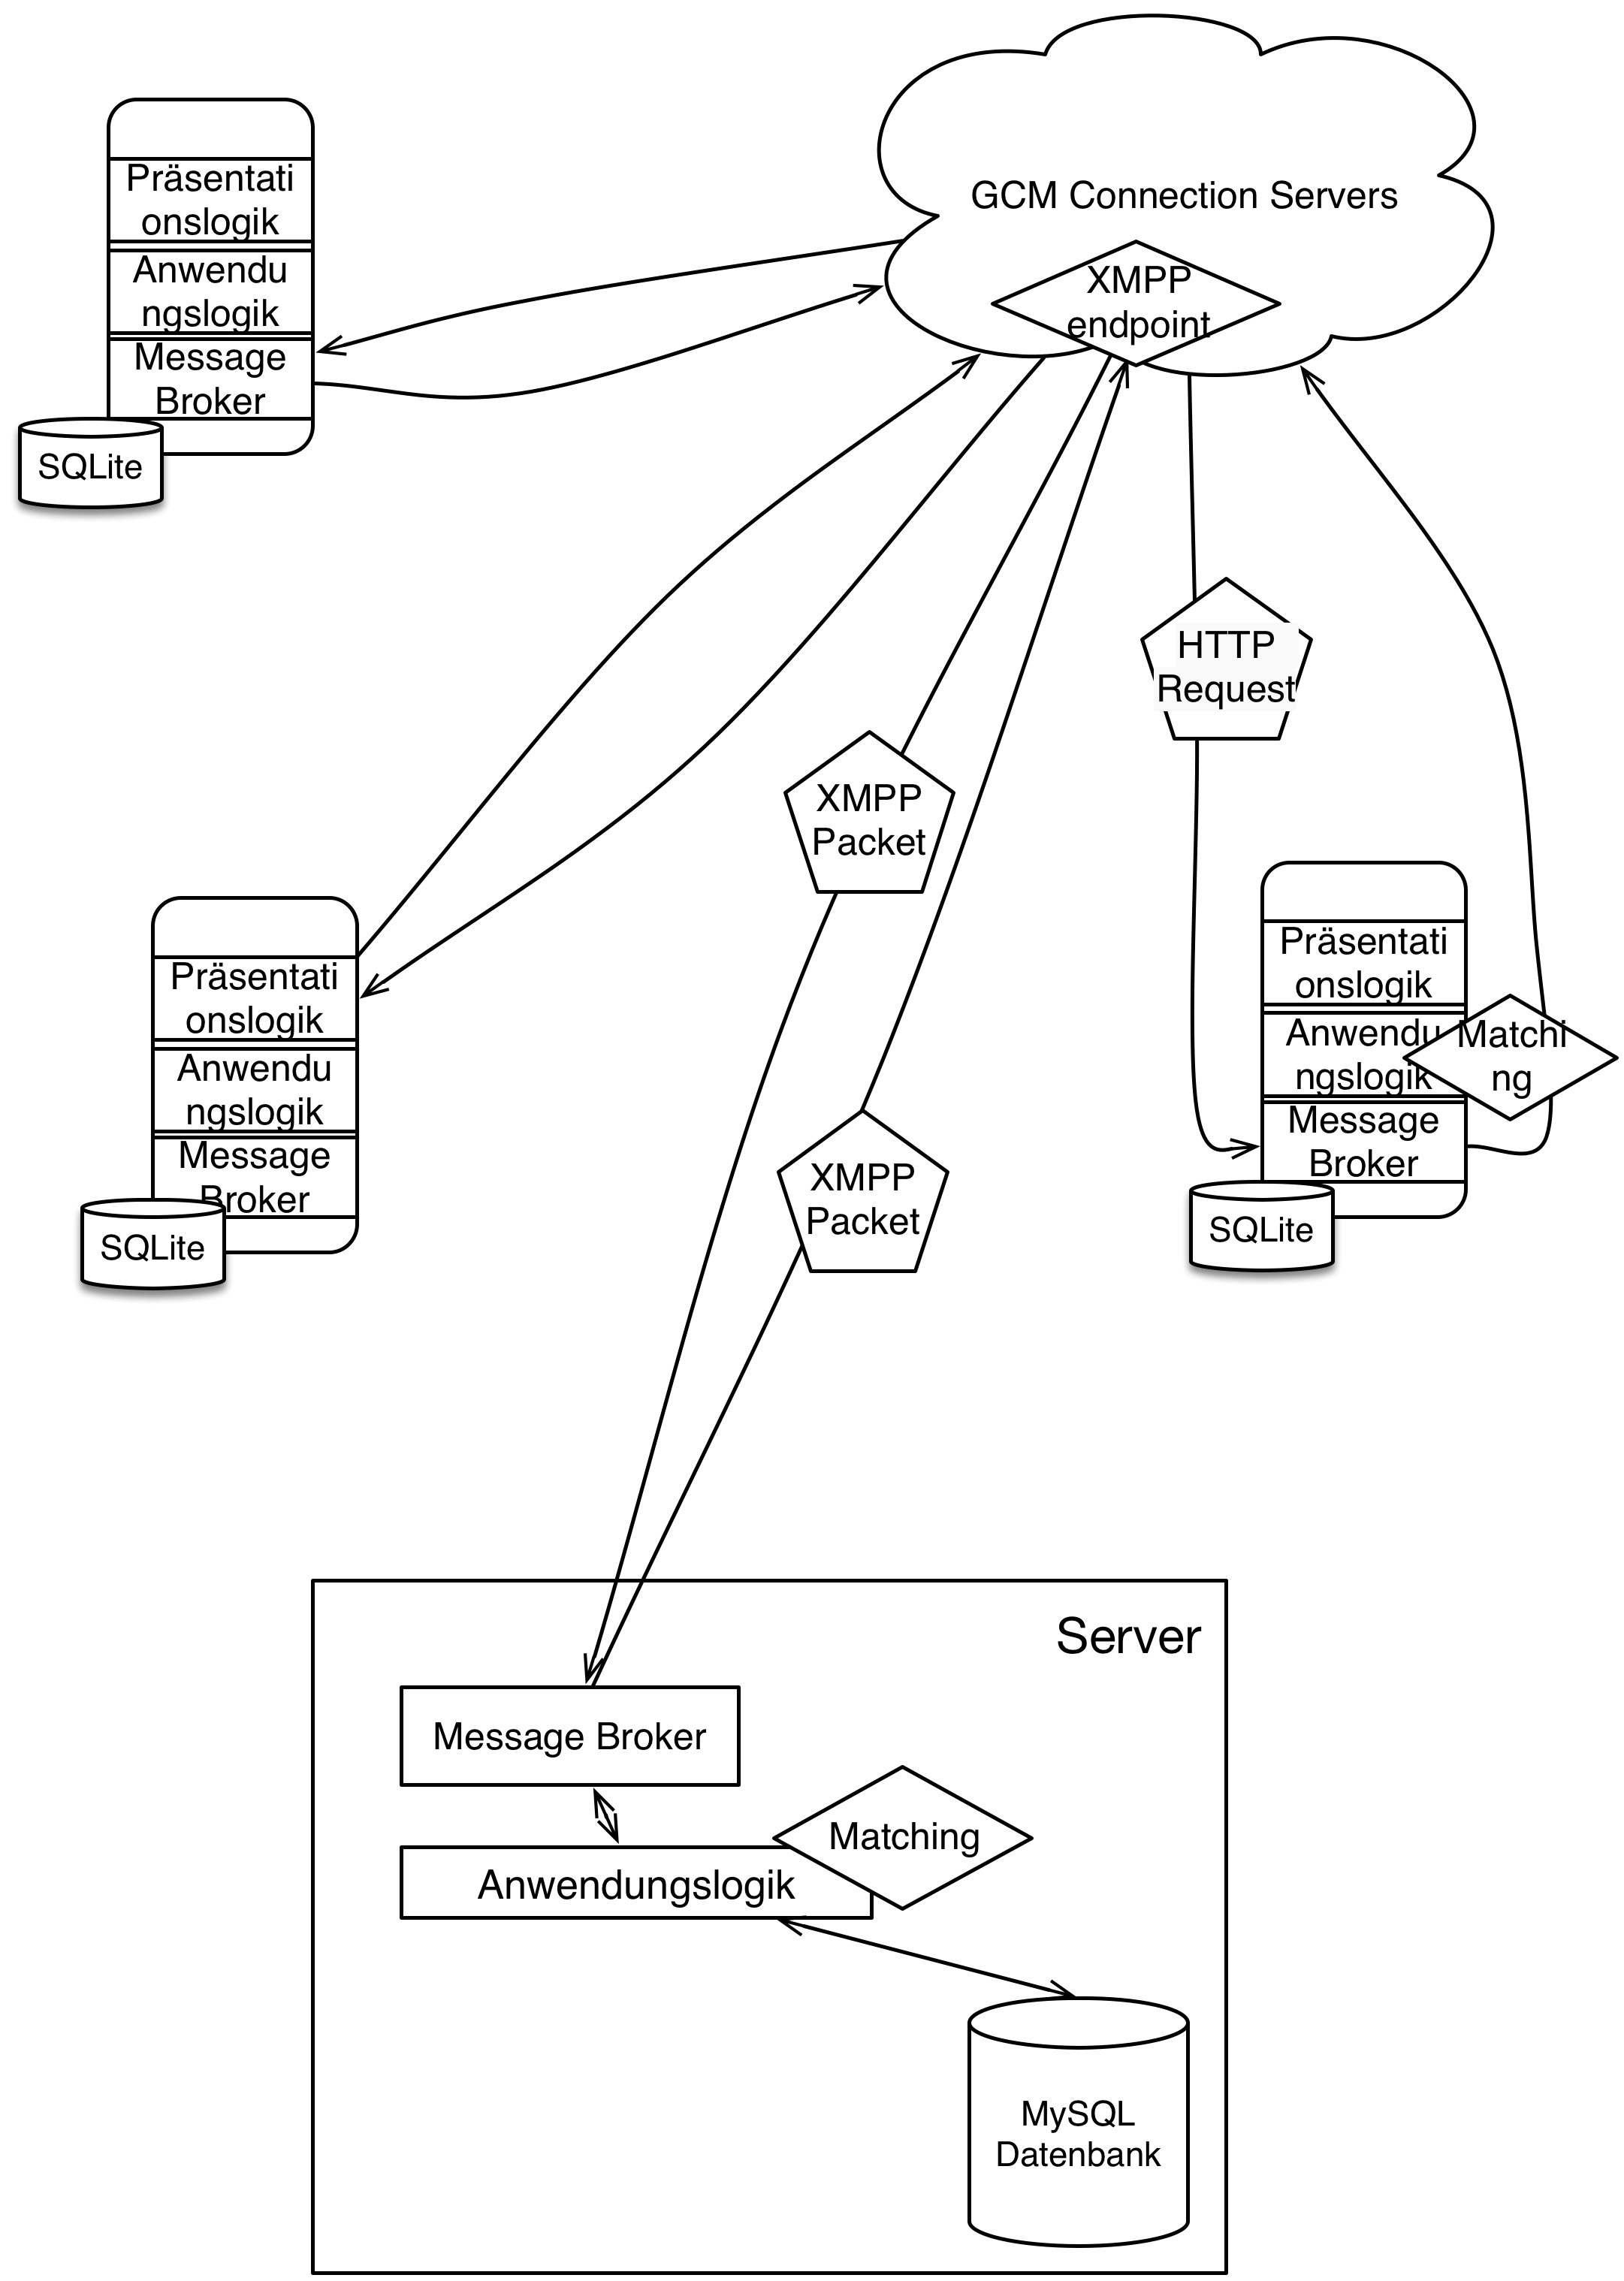
\includegraphics[width=0.85\textwidth]{./images/architekturneu.png}
	\caption{Systemarchitekur mit „GCM Cloud Connection Server“}
	\label{fg:gcmccsarchitecture}
\end{figure}
